\documentclass[letterpaper,11pt]{article}
\usepackage{graphicx}
\usepackage{listings}
\usepackage[super]{nth}
\usepackage[hyphens]{url}
\usepackage{hyperref}
\usepackage{amsmath}
\usepackage[makeroom]{cancel}
\usepackage[table]{xcolor}
\usepackage{comment}
\usepackage[space]{grffile}
\usepackage{csvsimple}
\usepackage{longtable}


\newcommand*{\srcPath}{../src}%

\lstset{
	basicstyle=\footnotesize,
	breaklines=true,
}

\begin{document}

\begin{titlepage}

\begin{center}

\Huge{Assignment 8}

\Large{CS 532:  Introduction to Web Science}

\Large{Spring 2017}

\Large{Grant Atkins}

\Large Finished on \today

\end{center}

\end{titlepage}

\newpage


% =================================
% First question
% =================================
\section*{1}

\subsection*{Question}

\begin{verbatim}
1.  Create a blog-term matrix.  Start by grabbing 100 blogs; include:

http://f-measure.blogspot.com/
http://ws-dl.blogspot.com/

and grab 98 more as per the method shown in class.  Note that this
method randomly chooses blogs and each student will separately do
this process, so it is unlikely that these 98 blogs will be shared
among students.  In other words, no sharing of blog data.  Upload
to github your code for grabbing the blogs and provide a list of
blog URIs, both in the report and in github.

Use the blog title as the identifier for each blog (and row of the
matrix).  Use the terms from every item/title (RSS) or entry/title
(Atom) for the columns of the matrix.  The values are the frequency
of occurrence.  Essentially you are replicating the format of the
"blogdata.txt" file included with the PCI book code.  Limit the
number of terms to the most "popular" (i.e., frequent) 1000 terms,
this is *after* the criteria on p. 32 (slide 7) has been satisfied.
Remember that blogs are paginated. 
\end{verbatim}

\clearpage
\subsection*{Answer}

To solve this problem I decided to write a shell script called \textbf{grabBlogs.sh} to retrieve the 98 random blogs as shown in Listing \ref{lst:grabBlogs}. The script utilizes mainly utilizes the curl and sort commands to solve the problem of retrieving unique blogs. The curl command is called 200 times with \url{http://www.blogger.com/next-blog?navBar=true&blogID=3471633091411211117} called each time to retrieve 200 blogs. I used 200 executions because I happened to get duplicate blogs on some occasions and 100 calls wouldn't be enough to satisfy the requirements of this problem. For each new blog I got I saved the contents of the html page to a html document with the an id of the current iteration in the range of 200. I saved this file id and the URI found inside a file called \textbf{blogList.txt} as shown in Listing \ref{lst:blogList}.

After 200 blogs were retrieved I used the sort command to find all unique blogs in the blog list file. Once this completed I had approximately 120 unique blogs. I then wrote a script in python 3.6 called \textbf{getFeed.py} as shown in Listing \ref{lst:getFeed} which parsed each html document saved using the library Beautiful soup which allowed me to search the document by an HTML `link` element to find the atom+xml feed of the blog \cite{beautifulsoupref}. I saved these feeds to a file called \textbf{feedList.txt} which was later cleaned for any blogs that did not have atom+xml feeds. Usually these were blogs that no longer existed. Any extra blogs above 100 were simply discarded.

Finally I proceeded to to write another python script called \textbf{generateFeedVector.py} shown in Listing \ref{lst:generateMat} which utilized the code provide by the Programming Collective Intelligence (PCI) book \cite{collectiveIntell}. This script was slightly modified to be usable for python 3.6 but also adding a limit to the amount of words the blog-term matrix allowed to a maximum of 1000 shown on line 65. I also didn't check for stop words when I retrieved the atom feeds, but I did check if words were stop words before creating the the matrix by using the nltk library's corpus of stop words shown on line 28. If a word was found to be a stop word according to their corpus it would not be added to the matrix. When this was completed it was saved to a file called \textbf{blogData.txt}.

 \lstinputlisting[frame=single,caption={Shell script to retrieve unique blogs},label=lst:grabBlogs,captionpos=b,numbers=left,showspaces=false,showstringspaces=false,basicstyle=\footnotesize]{\srcPath/grabBlogs.sh}

 \lstinputlisting[frame=single,caption={100 unique blogs collected},label=lst:blogList,captionpos=b,numbers=left,showspaces=false,showstringspaces=false,basicstyle=\footnotesize]{\srcPath/data/blogList.txt}

 \lstinputlisting[frame=single,caption={Python script to retrieve atom feeds of blogs},label=lst:getFeed,captionpos=b,numbers=left,showspaces=false,showstringspaces=false,basicstyle=\footnotesize]{\srcPath/getFeed.py}

 \lstinputlisting[frame=single,caption={Python script to generate blog-term matrix},label=lst:generateMat,captionpos=b,numbers=left,showspaces=false,showstringspaces=false,basicstyle=\footnotesize]{\srcPath/generateFeedVector.py}


\clearpage

% =================================
% Second question
% =================================

\section*{2}

\subsection*{Question}

\begin{verbatim}
2.  Create an ASCII and JPEG dendrogram that clusters (i.e., HAC)
the most similar blogs (see slides 12 & 13).  Include the JPEG in
your report and upload the ascii file to github (it will be too
unwieldy for inclusion in the report).
\end{verbatim}

\subsection*{Answer}

To solve this question I used the code provided by the Programming Collective Intelligence book to write a script in python 2.7 called \textbf{createClusters.py} as shown in Listing \ref{lst:createClusters} \cite{collectiveIntell}. This script has a method called \textit{createDendrogram} which utilizes the clusters.py file provided by the PCI book load the blog-term matrix created in question 1 to create a Hierarchical Clustering tree image, the dendrogram, as shown in Figure \ref{fig:dendro}. I also created an ASCII file named \textbf{q2ASCII.txt} to represent this tree structure in text which is available on my Github page \cite{github}.

 \begin{figure}[h]
 \centering
 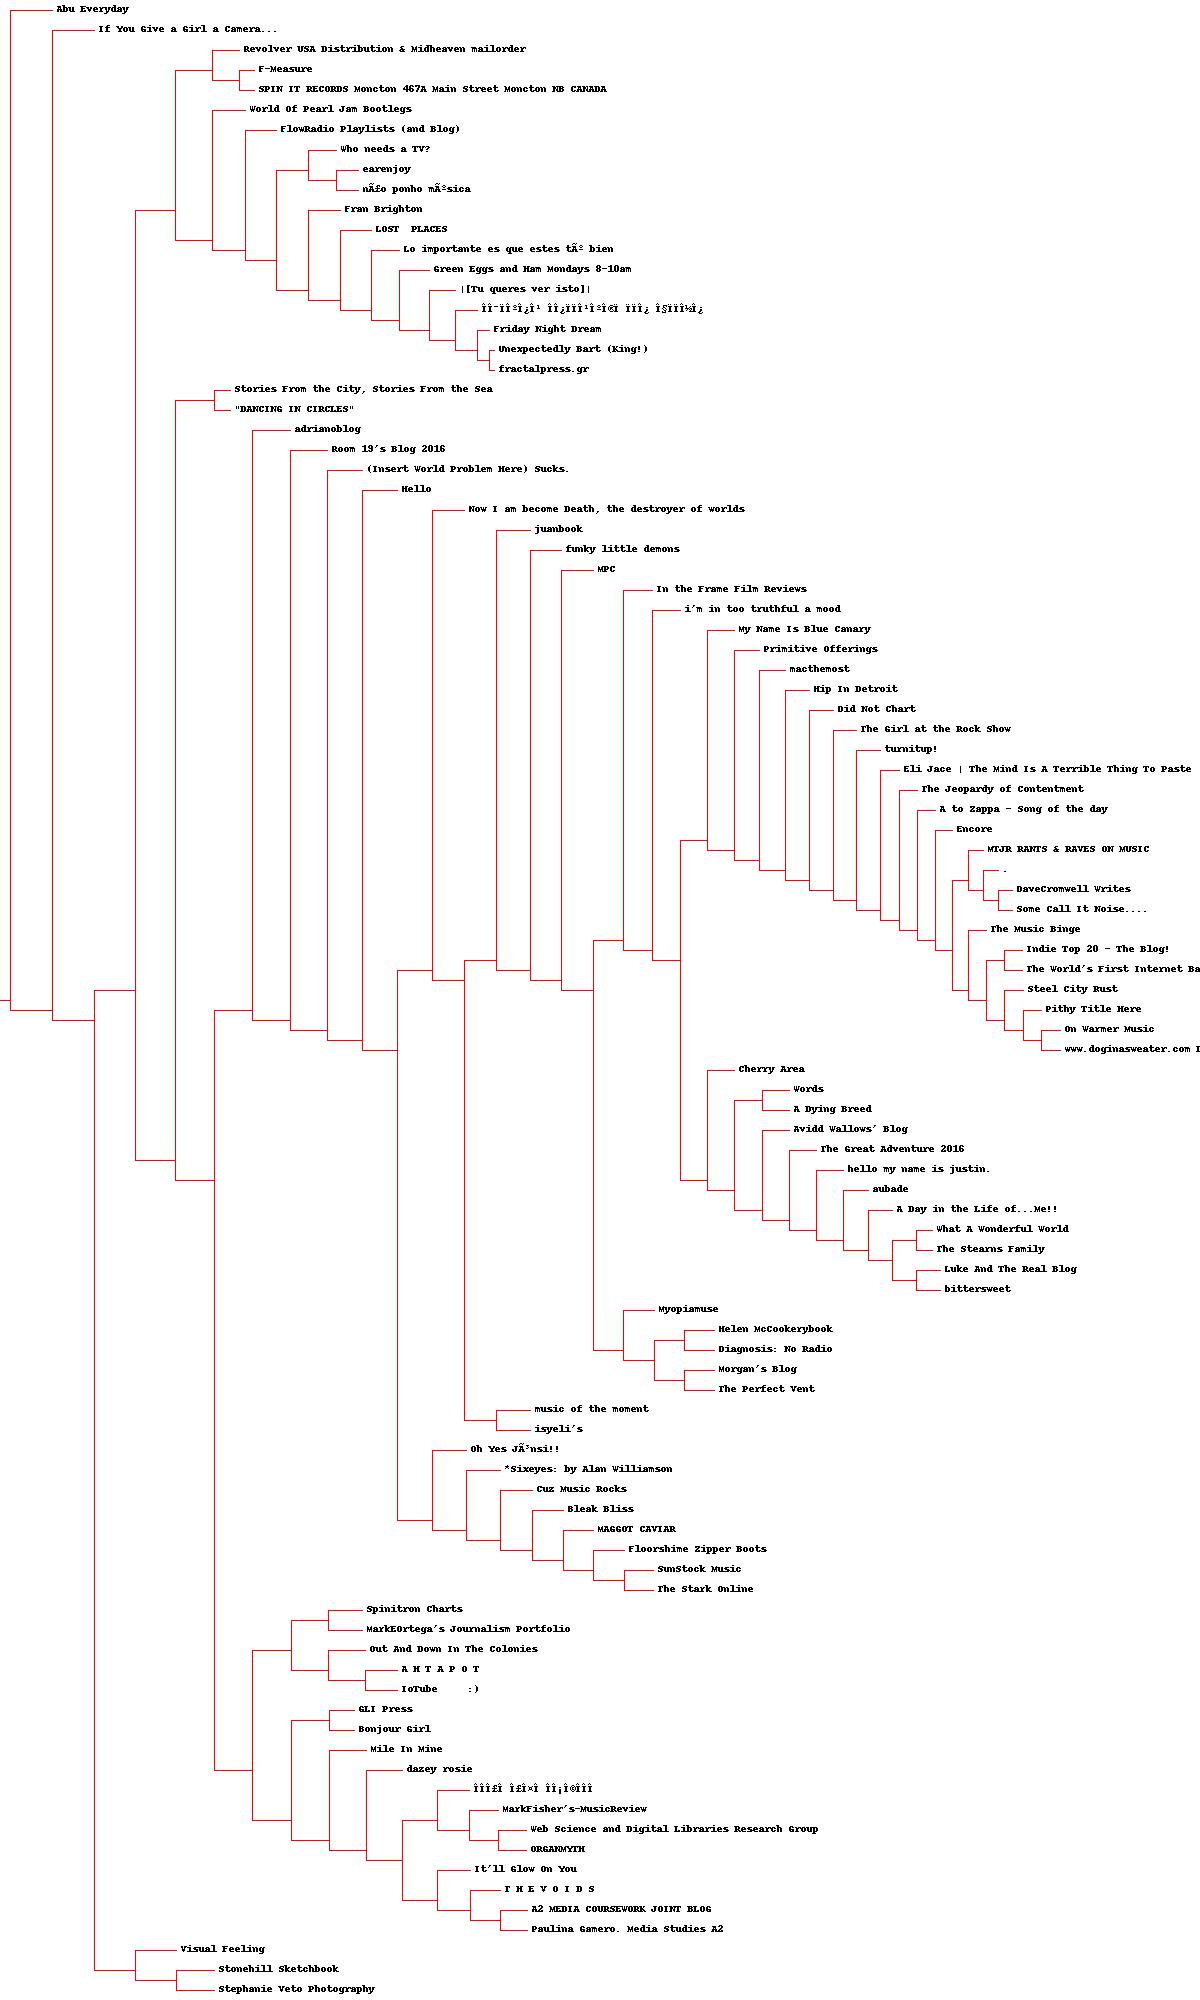
\includegraphics[scale=0.26]{q2Dendrogram}
 \caption{Dendrogram for blogs collected}
 \label{fig:dendro}
 \end{figure}

\clearpage

 \lstinputlisting[frame=single,caption={Python script to generate clusters with different approaches},label=lst:createClusters,captionpos=b,numbers=left,showspaces=false,showstringspaces=false,basicstyle=\footnotesize]{\srcPath/createClusters.py}

\clearpage

% =================================
% 3rd question
% =================================

\section*{3}

\subsection*{Question}

\begin{verbatim}
3.  Cluster the blogs using K-Means, using k=5,10,20. (see slide
18).  Print the values in each centroid, for each value of k.  How
many interations were required for each value of k?
\end{verbatim}

\subsection*{Answer}

To solve this question I again used the code provided by the Programming Collective Intelligence book as shown in Listing \ref{lst:createClusters} to create a method called \textit{kmeans} \cite{collectiveIntell}. The \textit{kmeans} method again reads my blog-term matrix and using the method \textit{kcluster} for the clusters.py library. I modified the \textit{kcluster} method to also return the iteration count so it could be saved along with the blog title. For each value of k I created a separate file named \textbf{kclut\_n.txt} where n is the value of k. For a k value of 5 it took 7 iterations with the values of each centroids shown in Listing \ref{lst:kclust5}. For a k value of 10 it took 5 iterations with the values of each centroids shown in Listing \ref{lst:kclust10}. For a k value of 20 it took 5 iterations with the values of each centroids shown in Listing \ref{lst:kclust20}.

 \lstinputlisting[frame=single,caption={K-means clustering with a value of 5},label=lst:kclust5,captionpos=b,numbers=left,showspaces=false,showstringspaces=false,basicstyle=\footnotesize]{\srcPath/data/kclust_5.txt}

 \lstinputlisting[frame=single,caption={K-means clustering with a value of 10},label=lst:kclust10,captionpos=b,numbers=left,showspaces=false,showstringspaces=false,basicstyle=\footnotesize]{\srcPath/data/kclust_10.txt}

 \lstinputlisting[frame=single,caption={K-means clustering with a value of 20},label=lst:kclust20,captionpos=b,numbers=left,showspaces=false,showstringspaces=false,basicstyle=\footnotesize]{\srcPath/data/kclust_20.txt}

\clearpage

% =================================
% 4th question
% =================================

\section*{4}

\subsection*{Question}

\begin{verbatim}
4.  Use MDS to create a JPEG of the blogs similar to slide 29 of the 
week 12 lecture.  How many iterations were required?
\end{verbatim}

\subsection*{Answer}

To solve this question I again used the code provided by the Programming Collective Intelligence book as shown in Listing \ref{lst:createClusters} to create a method called \textit{kmeans} \cite{collectiveIntell}. The \textit{kmeans} method again reads my blog-term matrix and using the method \textit{kcluster} for the clusters.py library. I modified the \textit{kcluster} method to also return the iteration count so it could be saved along with the blog title. 


\clearpage

% =================================
% Extra credit
% 5th question
% =================================

\section*{5}

\subsection*{Question}

\begin{verbatim}
5.  Re-run question 2, but this time with proper TFIDF calculations
instead of the hack discussed on slide 7 (p. 32).  Use the same 1000
words, but this time replace their frequency count with TFIDF scores
as computed in assignment #3.  Document the code, techniques,
methods, etc. used to generate these TFIDF values.  Upload the new
data file to github.

Compare and contrast the resulting dendrogram with the dendrogram
from question #2.

Note: ideally you would not reuse the same 1000 terms and instead
come up with TFIDF scores for all the terms and then choose the top
1000 from that list, but I'm trying to limit the amount of work
necessary.
\end{verbatim}

\subsection*{Answer}

\begin{center}
\Huge{NOT ATTEMPTED}
\end{center}


\clearpage

% =================================
% 6th question
% =================================

\section*{6}

\subsection*{Question}

\begin{verbatim}
6.  Re-run questions 1-4, but this time instead of using the 98 
"random" blogs, use 98 blogs that should be "similar" to:

http://f-measure.blogspot.com/
http://ws-dl.blogspot.com/

Choose approximately equal numbers for both blog sets (it doesn't
have to be a perfect 49-49 split, but it should be close).  
Explain in detail your strategy for locating these blogs.  

Compare and contrast the results from the 98 "random" blogs and 
the 98 "targeted" blogs. 
\end{verbatim}

\subsection*{Answer}

\begin{center}
\Huge{NOT ATTEMPTED}
\end{center}


\clearpage


% =================================
% Bibliography
% =================================

\begin{thebibliography}{9}
\bibitem{github}
Atkins, Grant. ``CS532 Assignment 8 Repository'' Github. N.p., 23 March 2017. Web. 23 March 2017.\url{https://github.com/grantat/cs532-s17/tree/master/assignments/A8}.
\bibitem{beautifulsoupref} 
Richardson, Leonard. "Beautiful Soup Documentation." Beautiful Soup Documentation - Beautiful Soup 4.4.0 Documentation. N.p., n.d. Web. 24 Jan. 2017. \url{https://www.crummy.com/software/BeautifulSoup/bs4/doc/}.
\bibitem{collectiveIntell}
Segaran, Toby. ``Programming Collective Intelligence''. O' Reilly, 2007. Web. 6 April 2017. \url{https://github.com/arthur-e/Programming-Collective-Intelligence}.
\end{thebibliography}

\end{document}